% !TeX root = ../../main.tex
\section{Powers of the first Hodge class}
\label{sec:s04}

We now compute the two corrections in Theorem~\ref{thm:lambda-one}.
The exact graph formula~\eqref{eq:s03:integrated-graph-formula} and
the normalization~\eqref{eq:s03:normalization-links} reduce the problem
to $Z_g(1)/F_g$. Theorem~\ref{thm:s03:graph-expansion} supplies an
expansion whose coefficients can be calculated by the summable core
rule~\eqref{eq:s03:coefficient-rule}. A core of complexity $q$ starts
at order $g^{-q}$: the leading term comes from $q=0$, the first
correction from $q=0,1$, and the second from $q=0,1,2$.

We first organize the correlated degrees at the two ends of each root
self-loop. These signed moments give the pure-loop corrections and,
after the small vertices are integrated, the corrections of the other
retained cores. We explain the coefficient mechanisms here and use
Appendix~\ref{sec:appendix-a} for their longer finite verification.
The final proof combines them with the absolute graph tail. Throughout
the calculation we normalize by $F_g$; the relative coefficients of
$Z_g/V_{g,0}$ will be distinguished explicitly.

% !TeX root = ../../main.tex
\subsection{Signed loop moments}
\label{subsec:s04:01}

An edge has one integration parameter, shared by its two flags in
\eqref{eq:s03:integrated-graph-formula}. For nonnegative integers
$a,b$ define its paired self-loop weight by
\begin{equation}\label{eq:s04:paired-weight}
 w_{ab}=\frac12\int_0^\alpha
       \frac{(-t/2)^{a+b}}{(2a+1)!(2b+1)!}\,\dd t
 =\frac{(-1)^{a+b}\pi^{2a+2b+2}}
       {(a+b+1)(2a+1)!(2b+1)!}.
\end{equation}
The factor $1/2$ accounts for exchange of the two branches of the loop. The denominator
$a+b+1$ records their common parameter; their weights do not factor
into independent endpoint weights.

For any nonnegative integer degree tuple $\mathbf d$, write
$D=|\mathbf d|$ and let
$m_a=\#\{i:d_i=a\}$ for $a=0,1,2$. Given $p\geq0$ ordered pairs
$(a_i,b_i)$, use the concatenated tuple
$\mathbf d=(a_1,b_1,\ldots,a_p,b_p)$, of length $2p$.
For a polynomial $\Phi$ in $p,D,m_0,m_1,m_2$ set
\begin{equation}\label{eq:s04:loop-functional}
 \mathcal L[\Phi]=e^{-S(1)}\sum_{p\geq0}\frac1{p!}
 \sum_{a_1,b_1,\ldots,a_p,b_p\geq0}
   \left(\prod_{i=1}^p w_{a_i b_i}\right)
       \Phi(p,D,m_0,m_1,m_2).
\end{equation}
The empty tuple has all five statistics zero. Together these symmetry
factors give $1/(2^pp!)$, exactly the automorphism factor for the
restored root loops. We also use the same series for the exponential
test functions in the next lemma.

The joint generator retains the low degrees needed at second order.
Let $v,x,z_0,z_1,z_2$ be independent complex moment parameters.

\begin{lmm}[Joint loop moments]\label{lmm:s04:loop-moments}
The functional~\eqref{eq:s04:loop-functional} is absolutely convergent
on polynomials, satisfies $\mathcal L[1]=1$, and has the entire
joint generating function
\begin{align}
 &\mathcal L\left[e^{vp+xD+\sum_{a=0}^2z_a m_a}\right]\notag\\
 &\quad=\exp\left\{\frac{e^v}{2}\int_0^\alpha
 \left[f(e^x t)+\sum_{a=0}^2(e^{z_a}-1)
               \frac{(-e^x t/2)^a}{(2a+1)!}\right]^2\dd t-S(1)\right\}.
 \label{eq:s04:joint-generator}
\end{align}
Every fixed moment is obtained by differentiating at zero. The
functional is signed, rather than a probability expectation.
\end{lmm}
\begin{prf}
For one edge the square selects its two endpoint degrees. Its
integral gives $w_{ab}$, the factors $e^x$ count their total degree,
and $e^{z_a}$ counts endpoints of degree $a$. Summing over $p$ with
$1/p!$ exponentiates this one-edge sum.

On compact sets of the moment parameters, the absolute endpoint
series are bounded by factorial series on the finite interval
$[0,\alpha]$. Their exponential sum over $p$ converges normally,
also after any fixed number of derivatives. This proves the
convergence and differentiation assertions. At zero parameters the
one-edge term is $\tfrac12\int_0^\alpha f(t)^2\dd t=S(1)$, proving
$\mathcal L[1]=1$.
\end{prf}

\begin{exm}[Two moments]
For a local complex variable $z$ near $1$, the degree generator of
one loop is
\[
 \sum_{a,b\geq0}w_{ab}z^{a+b}
 =\frac12\int_0^\alpha f(zt)^2\dd t=\frac{S(z)}z.
\]
Taking its Euler derivative gives the corresponding logarithmic
derivative of~\eqref{eq:s04:joint-generator}. Since
$S'(1)=\alpha f(\alpha)^2/2=0$, it follows that
\begin{equation}\label{eq:s04:representative-moments}
 \mathcal L[D]=-S(1),\qquad \mathcal L[m_0]=8.
\end{equation}
For the second identity, differentiation in $z_0$ gives
$\int_0^\alpha f(t)\dd t$. With $t=2y^2$ this is
$4\int_0^\pi\sin y\dd y=8$. Both endpoints contribute to this
derivative of the square. The remaining finite differentiation rules
and moment tables are given in Subsection~\ref{subsec:a:02}.
\end{exm}

% !TeX root = ../../main.tex
\subsection{The leading term and the first correction}
\label{subsec:s04:02}

% WORKFLOW-TODO: Write this subsection after the unit is assigned.

% !TeX root = ../../main.tex
\subsection{The second correction}
\label{subsec:s04:03}

For $q=0,1,2$, let $\left.Z_g(1)/F_g\right|_q$ denote the
contribution of graphs with a large vertex and core complexity $q$.
Define constants $Q_{q,r}$, for integers $0\leq r\leq2-q$, by
\begin{equation}\label{eq:s04:absolute-groups}
 \left.\frac{Z_g(1)}{F_g}\right|_q
 =\frac{e^{S(1)}}{\sqrt\pi}\,g^{-q}
       \left(\sum_{r=0}^{2-q}\frac{Q_{q,r}}{g^r}
                       +O(g^{-(3-q)})\right).
\end{equation}
Their existence follows from the finite-core expansion and its
summable remainder, multiplied by the absolute volume expansion.
The preceding subsection gives $Q_{0,0}=1$ and
$Q_{0,1}+Q_{1,0}=9/8$. These are coefficients of $Z_g(1)/F_g$.
The functions $\gamma_r$ in Theorem~\ref{thm:s03:graph-expansion}
are the coefficients in the expansion normalized by $V_{g,0}$.

At second order the pure-loop core requires both profiles and the
absolute second volume coefficient. Complexity-one cores require
their first corrections, and complexity-two cores only their leading
small-vertex integrals. We explain these three inputs separately;
Appendix~\ref{sec:appendix-a} supplies the full finite evaluations.

\begin{prp}[The second correction]\label{prp:s04:second-correction}
The absolute groups are
\begin{align}
 Q_{0,2}&=\frac{43}{288}-\frac{469}{36\pi^2}
                                      +\frac{5665}{72\pi^4},\notag\\
 Q_{1,1}&=\frac{73}{288}-\frac{1843}{144\pi^2}
                                      -\frac{6565}{36\pi^4},\notag\\
 Q_{2,0}&=\frac{1849}{1152}+\frac{3737}{144\pi^2}
                                      +\frac{7465}{72\pi^4}.
 \label{eq:s04:second-groups}
\end{align}
In particular,
\begin{equation}\label{eq:s04:second-total}
 Q_{0,2}+Q_{1,1}+Q_{2,0}=\frac{257}{128}+\frac1{8\pi^2}.
\end{equation}
\end{prp}
\begin{prf}
For the pure-loop vertex expand the absolute volume one order further
than~\eqref{eq:s04:pure-loop-volume}. Its second coefficient is
\[
 \frac{3p^2}{8}+\frac{3p}{2}c_1(2p)+c_2(2p).
\]
Here $3p^2/8$ is the next square-root correction, and the middle
term combines the shift from $g-p$ to $g$ with the first square-root
term. Multiplication by the profile in complexity $2g-2$ gives
\begin{equation}\label{eq:s04:q-zero-mechanism}
\begin{aligned}
 Q_{0,2}=\mathcal L\biggl[&\frac{3p^2}{8}
   +\frac{3p}{2}c_1(2p)+c_2(2p)\\
 &+\frac12\left(1+\frac p2+c_1(2p)\right)e_{2p,1}(\mathbf d)
       +\frac14e_{2p,2}(\mathbf d)\biggr].
\end{aligned}
\end{equation}
The extra $1$ multiplying the first profile comes from
$(2g-2)^{-1}=(2g)^{-1}+(2g^2)^{-1}+O(g^{-3})$.
The argument $\mathbf d$ is the concatenated loop tuple of
Subsection~\ref{subsec:s04:01}. The complete second profile retains
both $m_1$ and $m_2$. Proposition~\ref{prp:a:c-two} reconstructs
$c_2(n)$ from the exact intersection recursions, and
Proposition~\ref{prp:a:pure-loops} evaluates this polynomial moment.
It gives the first row of~\eqref{eq:s04:second-groups}.

For a complexity-one core, let $n_0$ be its root valence and
$c=(n_0+1)/2$ its genus loss before root loops are restored.
Here $n_0$ is either $1$ or $3$. Append the nonnegative connector
degrees $\mathbf d_{\rm c}$, of length $n_0$, to the loop tuple.
The first absolute correction before connector integration is
\begin{equation}\label{eq:s04:q-one-mechanism}
 \frac32+\frac{p+c}{2}+c_1(2p+n_0)
       +\frac12e_{2p+n_0,1}(\mathbf d,\mathbf d_{\rm c}).
\end{equation}
The $3/2$ comes from the complexity-one factorial ratio; the next
term is the root's square-root genus correction. Average this
polynomial over its loops, then take the raw connector moments.

For a local complex degree parameter $x$ near $1$, the elliptic
connector generator is the unscaled integral
\[
 \int_0^\alpha W^{\rm WP}_{1,1}(t)f(xt)\,\dd t.
\]
Its Euler derivatives at $x=1$ give the degree moments, keeping
$W^{\rm WP}_{1,1}(t)$ fixed. There is no loop factor $1/2$ on a
connector. The rational connector uses the same integral with
$W^{\rm WP}_{0,3}=1$. Proposition~\ref{prp:a:q-one} performs these
finite integrations for the three cores, with their automorphism
orders $1,6,2$ as above. Their correction sum is the second row
of~\eqref{eq:s04:second-groups}.

For $q=2$, each core has one small vertex of complexity two or two
small vertices of complexity one. Thus only the four polynomials of
Lemma~\ref{lmm:a:small-vertices} are needed. The leading root-volume
factor is $(8\pi^2g)^{-2}$, and its flags again contribute $f$.
Root-loop resummation gives $e^{S(1)}$. Lemmas
\ref{lmm:a:core-enumeration} and~\ref{lmm:a:core-integration} supply
the complete list of thirteen cores and their exact integration rule.
Their individual integrals are listed in Subsection~\ref{subsec:a:04};
Proposition~\ref{prp:a:finite-summary} gives the third row.

The rational, $\pi^{-2}$ and $\pi^{-4}$ coefficients are, respectively,
\begin{align*}
 \frac{43}{288}+\frac{73}{288}+\frac{1849}{1152}
   &=\frac{257}{128},\\
 -\frac{469}{36}-\frac{1843}{144}+\frac{3737}{144}
   &=\frac18,\\
 \frac{5665-2\cdot6565+7465}{72}&=0.
\end{align*}
These three sums prove~\eqref{eq:s04:second-total}.
\end{prf}

\begin{exm}[A complexity-two core]
Consider the rational four-valent small vertex with two connectors
and one self-loop:
\begin{center}
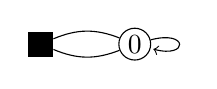
\begin{tikzpicture}[x=1.2cm]
 \node[rectangle,fill,minimum size=3.2mm,inner sep=0pt] (v0) at (0,0) {};
 \node[circle,draw,inner sep=1.2pt] (v1) at (1,0) {$0$};
 \draw (v0) to[bend left=22] (v1);
 \draw (v0) to[bend right=22] (v1);
 \draw (v1) edge[loop right] (v1);
\end{tikzpicture}
\end{center}
Its automorphism order is $2!\cdot2=4$. Write $t_1,t_2$ for the
connector variables and $s$ for the small loop variable, each in
$[0,\alpha]$. Its vertex polynomial is
$2\pi^2-t_1-t_2-2s$; the two flags of that loop both use $s$.
Integration in $s$ leaves $-\alpha(t_1+t_2)$, so its contribution
to $Q_{2,0}$ is
\begin{equation}\label{eq:s04:q-two-example}
 -\frac{\alpha}{4(8\pi^2)^2}\int_{[0,\alpha]^2}
 f(t_1)f(t_2)(t_1+t_2)\,\dd t_1\dd t_2
 =-1+\frac4{\pi^2}.
\end{equation}
The two connector moments were evaluated in the preceding subsection.
This is core $2.1$ of the appendix table. Its negative contribution
comes from the exact negative-psi polynomial.
\end{exm}

\begin{rmk}[Absolute normalization]
The $Q_{q,r}$ include the absolute WP corrections. In particular
the relative coefficient of Theorem~\ref{thm:s03:graph-expansion}
satisfies
\[
 e^{-S(1)}\gamma_1(1)=\frac98-c_1(0).
\]
At second order the conversion also includes $c_2(0)$ and the product
of the two first coefficients, as explained in
Subsection~\ref{subsec:a:02}.
\end{rmk}

\begin{rmk}[The absolute volume input]
The proof of Proposition~\ref{prp:a:c-two} uses the exact recursions
of \cite[Section~2]{MZ15} and \cite[Theorem~4.3]{HMT25}. Its
adjacent-genus comparison uses the actual fixed-marking expansion
through order three, so the unknown third volume coefficient cancels.
The result agrees with \cite[(6.10)]{EGGLS24}, derived there under
the resurgence assumption in Section~6.1 before (6.6). That conditional
prediction is a comparison after the reconstruction and is not a
proof input here.
\end{rmk}

% !TeX root = ../../main.tex
\subsection{Proof of Theorem 1.1}
\label{subsec:s04:04}

% WORKFLOW-TODO: Write this subsection after the unit is assigned.

